\documentclass{beamer}

% !TEX root = ./main.tex
% The above line is a magic comment that tells text editors which file to compile.

\documentclass{beamer}
\usepackage[utf8]{inputenc}
\usepackage{hyperref}
\usepackage{amsmath}
\usepackage{cleveref}
\usepackage{adjustbox}
\usepackage{mathtools}
\usepackage{dsfont}
\usepackage{xcolor}
\usepackage{amsthm}

\usepackage{tikz}
% \usetikzlibrary{arrows.meta}
% \usetikzlibrary{shapes}
% \usetikzlibrary{calc}
% \usetikzlibrary{math}
% \usetikzlibrary{decorations.pathreplacing,calligraphy}
% \usepackage{pgffor}

% \usepackage{algorithm}
% \usepackage{algpseudocode}

\usepackage{macros}
\usepackage{domainmacros}
%%%%%%%%%%
% Beamer %
%%%%%%%%%%

\definecolor{cPurple}{RGB}{124, 0, 133}
\definecolor{cBlue}{RGB}{56, 0, 138}
\definecolor{cRed}{RGB}{180, 0, 60}
\definecolor{cGreen}{RGB}{0, 156, 27}

\usetheme[sectionpage = none, subsectionpage = simple]{metropolis}
\usecolortheme{seahorse}

\usebeamercolor{normal text}
\usebeamercolor{background canvas}

\setbeamercolor{alerted text}{fg=cPurple}

\setbeamertemplate{footline}{%
      \raisebox{8pt}{\makebox[\paperwidth]{\scriptsize \hfill \insertframenumber/\inserttotalframenumber \hspace{5pt}}}}

% \setbeamertemplate{footline}{\raisebox{8pt}{\hfill \insertframenumber/\inserttotalframenumber \hspace{5pt}}}

% \setbeamertemplate{footline}{%
%       \raisebox{8pt}{\makebox[\paperwidth]{\scriptsize \hspace{5pt}  TCS101 \hfill \insertframenumber/\inserttotalframenumber \hfill CC-BY-SA \hspace{5pt}}}}

\beamertemplatenavigationsymbolsempty

\title[RBSR]{Range-Based Set Reconciliation}
\author{Aljoscha Meyer}
\date{}

\begin{document}

\frame{\titlepage}

\begin{frame}{Set Reconciliation}
    \begin{itemize}
        \item set union over a network
        \item between (exactly) two machines
        \item unstructured data
        \item no shared state or history
    \end{itemize}
\end{frame}

\begin{frame}{Trivial Reconciliation}
    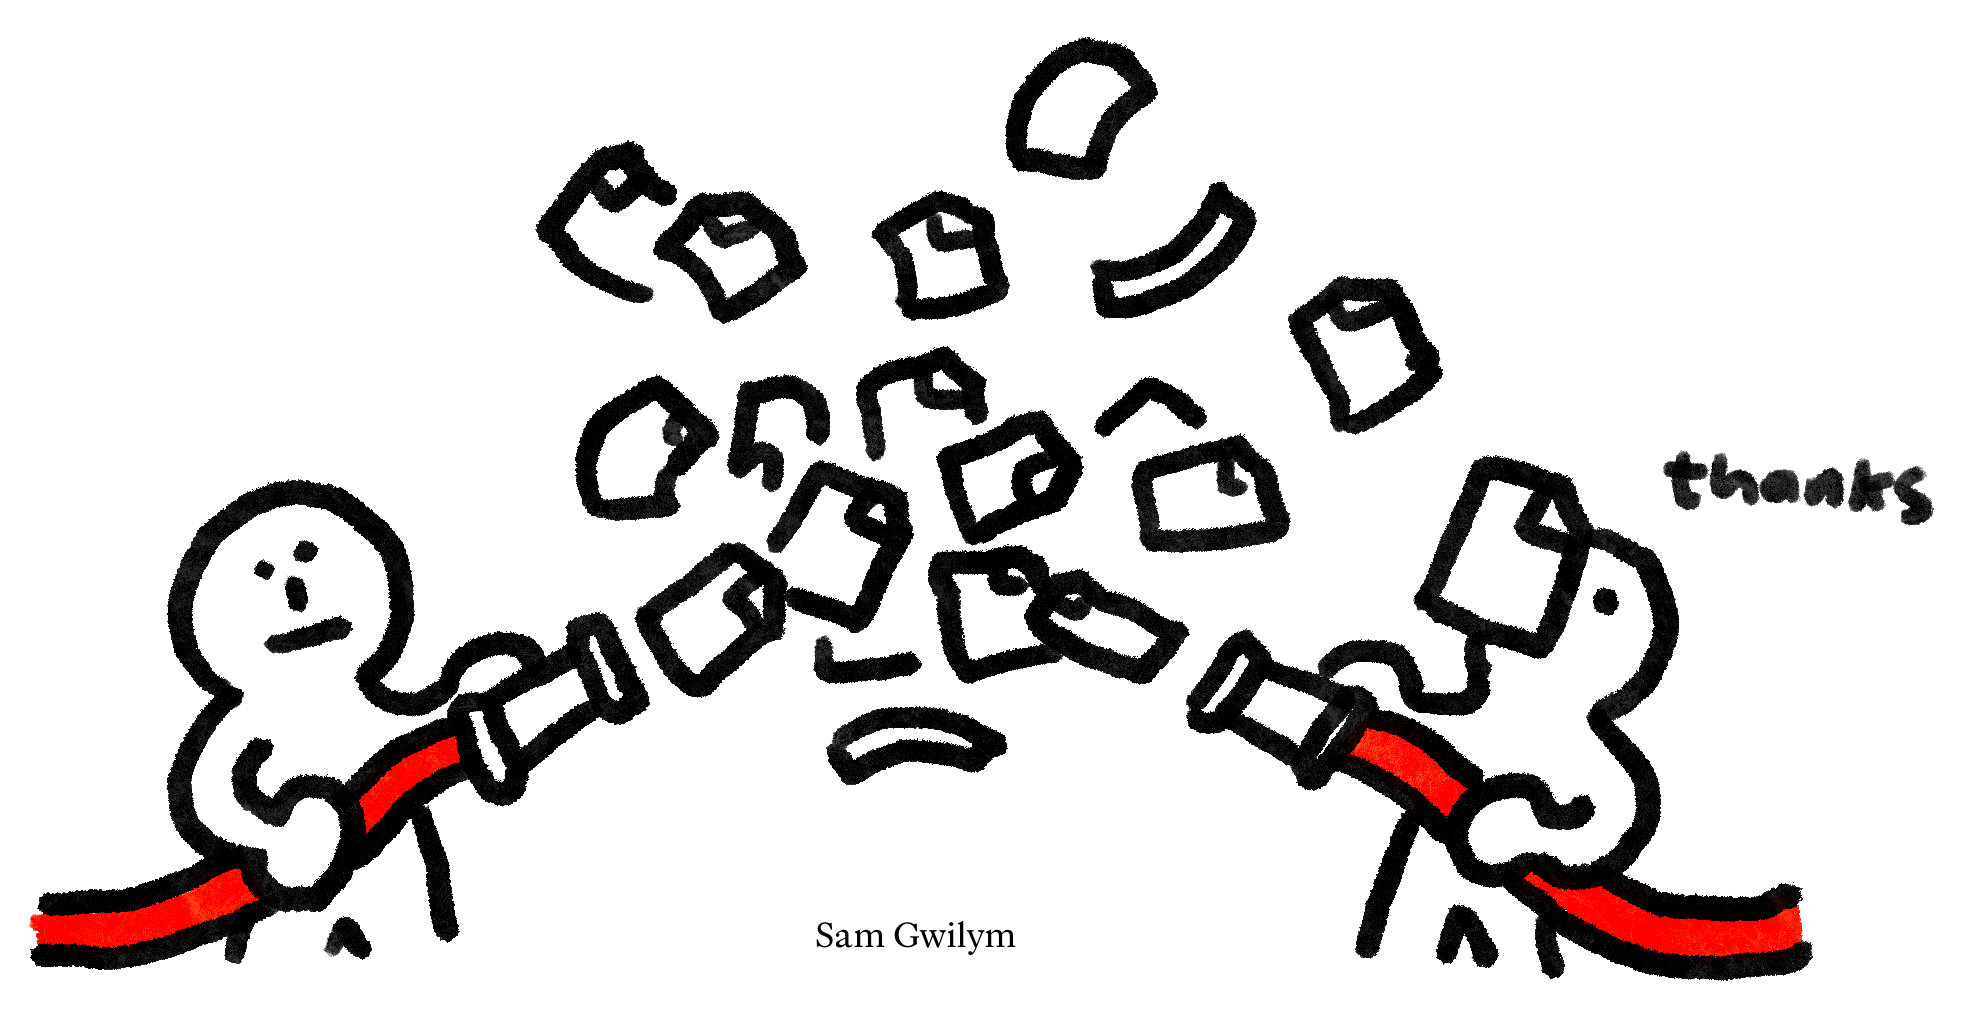
\includegraphics[keepaspectratio=true,width=11.4cm]{trivial_sync.png}
\end{frame}

\begin{frame}{Model and Analysis}
    \begin{itemize}
        \item Alfie and Betty talk over a network
        \item reliable communication, rounds of unit length, unlimited bandwidth
        \item probabilistic solutions \pause
        \item $n$: size of the union
        \item $n_{\triangle}$: size of the symmetric difference
    \end{itemize}
\end{frame}

\begin{frame}{Model and Analysis}
    \begin{itemize}
        \item roundtrips
        \item communicated bytes
        \item computation time per reconciliation session
        \item computation space per reconciliation session
        \item computation time per item
        \item computation space per item
    \end{itemize}
\end{frame}

\begin{frame}{P2P Reconciliation}
    Peer-to-peer systems:
    \begin{itemize}
        \item iterating over local set infeasible
        \item loading local set into memory infeasible
        \item some peers are out to get us
    \end{itemize}

    \pause

    $\implies$ traditional approaches don't work
\end{frame}

\begin{frame}{Range-Based Set Reconciliation}
    $X_{\alpha} \defeq \{\exampleb, \examplec, \exampled, \examplee, \examplef, \exampleh \}$
    \hfill
    $X_{\beta} \defeq \{\examplea, \examplee, \examplef, \exampleg\}$
    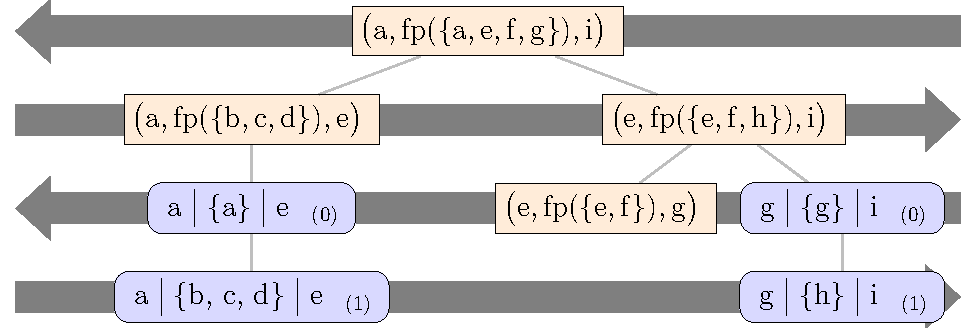
\includegraphics[keepaspectratio=true,width=11.4cm]{examplerun.pdf}

    % \item hence relax to logarithmic number of rounds
    % \item divide-and-conquer -> explain rbsr
    % \item complexity analysis
\end{frame}

\begin{frame}{Some Nice Properties}
    \begin{itemize}
        \item reasonably efficient: $\complexity{\min(n_{\triangle} \cdot \log(n), n)}$ bytes communication, $\complexity{1}$ working memory
        \item arbitrary recursion anchor protocols
        \item arbitrary partition techniques \pause
        \item but: linear computation times
    \end{itemize}
\end{frame}

% \begin{frame}{}
%     \begin{itemize}
%         \item two issues, start with the subtle one
%         \item deadlock
%         \item solution
%         \item analysis and model
%     \end{itemize}
% \end{frame}

\begin{frame}{Reducing Computation Times}
    \begin{itemize}
        \item Step 1: Put a Merkle tree on it
        \item Step 2: ???
        \item Step 3: Profit
    \end{itemize}
\end{frame}

\begin{frame}{}
    
\end{frame}



\begin{itemize}
    \item not-so-subtle: linear computation times
    \item first approach (kinda-acceptable but not really): put a Merkle tree on it
    \item explain Merkle trees
    \item different trees of the same data leads to different root labels -> history-independent data structure
    \item cannot fingerprint arbitrary ranges -> let tree shape guide reconciliation
    \item MSTs
    \item problem 1: everyone has to use that one representation
    \item problem 2: adversarial trees
    \item blueskies...
\end{itemize}

\begin{itemize}
    \item let's backtrack and solve the first problem -> associativity
    \item example tree (using counts, then hashes)
    \item definition
    \item arbitrary ranges: collections of maximal subtrees, complexity analysis
    \item successive ranges yay
\end{itemize}

\begin{itemize}
    \item this gives us worst-case bounds on roundtrips
    \item implementation independence
    \item more datastructure-neutral formulation: monoids
    \item paper actually uses different data structure, also B-trees, skip lists, radix trees, no data structure, ... and all interoperable
\end{itemize}

\begin{itemize}
    \item malicious adversaries: active vs passive
    \item even passive finds collisions in relatively small sets
    \item but: collision must actually affect a session -> brittle, and randomization ftw
    \item But what if there are many collisions? -> collision-resistant hash functions
\end{itemize}

\begin{itemize}
    \item must always lift into the monoid with a secure hash function. Interesting part is the selection of the monoid
    \item bellare: xor, addition, multiplication, vectorized addition (lattices)
    \item multiset homomorphic hashing adds rsa and elliptic curves
    \item we are weaker: homomorphism-flavored characterization
    \item in particular, no need for commutativity (because we use search trees) -> matrix multiplication -> cayley hashes
    \item Don't know anything else, but cayley still has unnecesary structure, as we do not need inverses
\end{itemize}

\begin{itemize}
    \item conclusion: first non-trivial reconciliation algorithm to work in resource-constrained settings and adversarial environments
    \item also: comparatively simple -> had multiple open source developers reach out to me
\end{itemize}
% \end{frame}

\end{document}
